% !TeX root = ../praktikum.tex
% !TeX encoding = UTF-8
% !Tex spellcheck = de_DE

Der Laserstrahl eines \textit{LD: Mitsubishi ML101J27} cw- Lasers, betrieben mit 90,3 mA bei $18^\circ C$, mit einer Wellenlänge von 660nm und einer maximalen Leistung von 35 mW wird in eine Leitungsfaser eingekoppelt. \\

\begin{figure} [h]
\centering
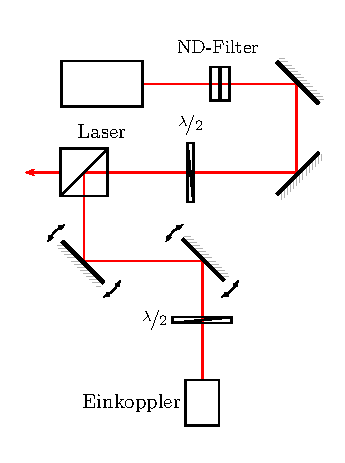
\includegraphics[width=0.5\linewidth]{graphs/versuchsaufbau/lasereinheit}
\caption{Schematischer Strahlungsaufbau zwischen Laser und Fasereinkopplung. Mit Hilfe der $\frac{\lambda}{2}$- Platte und des Strahlteilers dahinter kann die Intensität des Laserstrahls eingestellt werden. Der zweite Strahl nach dem Strahlteiler dient zum parallelen Durchführen des Versuchs durch eine zweite Gruppe und wird daher nicht weiter betrachtet.}
\label{fig:lasereinheit}
\end{figure}
\\
Der Faserkopplungsaufbau (siehe Abbildung \ref{fig:lasereinheit}) wird nicht selbst aufgebaut, sondern lediglich optimiert. Hierzu wird ein Laserpointer an dem noch freien Ende der Faser angebracht und vor dem Einkoppler mithilfe der Spiegel eine optimale Überlagerung der beiden Signale eingestellt. \\
Anschließend betrachtet man das eingekoppelte Signal am Ende der Faser, um dessen Leistung weiter zu optimieren. Dies erfolgt zunächst mit dem bloßen Auge und anschließend mit einem Powermeter, welches an ein Oszilloskop angeschlossen wird, um schnelle Änderungen der gemessenen Lichtleistung besser sichtbar zu machen. Es wird ein Optimum der Fasereinkopplung möglichst genau eingestellt. 



